% das Papierformat zuerst
\documentclass[a4paper, 12pt]{article}

\usepackage{fancyvrb}

\usepackage[pdftex]{graphicx}

\usepackage[left=35mm,right=35mm,top=25mm,bottom=25mm]{geometry}

\newenvironment{mySourceCode}
{\begin{list}{}{\setlength{\leftmargin}{2em}}\item\scriptsize\bfseries}
{\end{list}}

% hier beginnt das Dokument
\begin{document}

% =======================================================================
% Titelseite

\begin{center}
\Large{University of applied Sciences Wedel}
\end{center}

\begin{center}
\Large{Departement: Computer Science}
\end{center}

% nicht zu parsende Zeichen
\begin{verbatim}





\end{verbatim}

\begin{center}
\textbf{\LARGE{Term Paper}}
\end{center}

% nicht zu parsende Zeichen
\begin{verbatim}


\end{verbatim}

\begin{center}
\textbf{\large{Course of studies: Computer Science and Digital Media}}
\end{center}

% nicht zu parsende Zeichen
\begin{verbatim}












\end{verbatim}

\begin{flushleft}
\begin{tabular}{llll}

\textbf{Subject:}
& & & Backdoors in Software Implementations
\\
\\
\textbf{Submitted by:}
& & & Maurice Tollmien -- minf8914@fh-wedel.de
\\
\\
\textbf{Submitted at:}
& & & 29/11/2012
\\
\\
\textbf{Advisor:}
& & & Prof. Dr. Beuster



\end{tabular}
\end{flushleft}


\newpage

% =======================================================================
% Inhaltsverzeichnis

\tableofcontents
\newpage

% -----------------------------------------------------------------------
% Introduction

\section{Introduction}


In our world todftfdsdsadsadsyfdrrtuhlöltrtay, everything is controlled and monitored by computer systems. Private people as well as big companies, banks and the military are depending on computer systems that get larger and more complex every day.
But the more computer systems are needed to get our life sorted, the more important it is to obtain a high security level on every bit we shift, every interface that connects different computer systems and, of course, every possible connection to the world wide web.

Taking current circumstances into account, it is very important to deal with threats coming from unknown directions, trying to get in control of secured computer systems.

Maliciously modified devices are just one example of how real these threats already are. For example Apple sold iPods, infected with the RavMonE-Virus in the year 2006[1]. Quite recently Seagate, a company from Taiwan, was shipping hard drives, that had a Trojan horse on board, that sent private information about the person's computer back to the remote attacker[2].

%And there are a lot more examples. We will get back to this with specific examples of Backdoors in Softwareimplementations in Chapter 3 [Backdoor Compiler] and 4 [Examples of Backdoors].

\subsection{Scope of Study}

In this article I will mainly present and discuss a special form of the trojan horse, the Backdoor.

I will start by explaining what different kind of Backdoors exist and how they differ from each other.
After defining the topic of this paper, we will focus on a special kind of Backdoor, the Backdoor compiler, and explain why this not widely known type of trojan horse could be of particular importance regarding securing computer systems.

After demonstrating how this kind of Backdoor could be implemented, it is very important to also look at ways and possiblities to take action against it. Or at least find out whether `we' are infected or not.

By looking at options to track the Backdoor down and clean systems from it, if they are infected, we will discuss several ways that will help us to counter this particular threat and take actions against it.

Because the Backdoor will affect compilers that means, to talk about compiler output testing and whether it is correct or not. 

\newpage
 
% -----------------------------------------------------------------------
% Backdoors - A definition
\ 
\section{Backdoors - A definition}

$ \frac{Zaehler}{Nenner} $


\newpage
The first step of hacking a computer system, breaking in, taking control, just do some damage or tie computer systems up is always to get into their system first.
There are different ways to get into a computer system. The most simple way would be, to get the user to actually start your malicious program himself by convincing him, that your program is useful, funny, interesting or similar.

But much more important to any hacker is not a single break in, damage and leave, but to get continuous access rights to system functionality, so he could use it whenever he wants. This is widely called a Backdoor.

Generally a Backdoor is called everything, that bypasses the volitional way of communication between different interfaces[13].

To give examples, a Backdoor could be a possibility to access a computer via a network system like the internet without you or your firewall noticing. Another one could be a hardcoded password in the login function of an operating system which logs the attacker in with root privilege.

Leading from these examples you see, that Backdoors could be of different kinds. The most simple Backdoor is, as mentioned, a hardcoded password, which the software designer coded in[13]. This kind of Backdoor is mostly not implemented with bad intentions in mind, but to gain control in critical situations. There are also types of Backdoors that were not even designed on purpose. A simple example of that could be a programming mistake, that might give access to a system, which was probably not intended. These errors happen, but can fortunately not be used as a Backdoor most of the time.

All kinds of Backdoors mentioned above can be characterized as either a symmetric Backdoor or an asymmetric Backdoor.

\newpage

\subsection{Symmetric Backdoors}

The symmetric Backdoor is a characterization of the most types of Backdoors that we know.

It simply means that whoever finds the Backdoor, can use it. The example, a hardcoded password in the login-command, is such a Backdoor. That means, whoever finds out about the secret password, can then use it, to get access to the system[14].

\subsection{Asymmetric Backdoors}

In contrast to the symmetric Backdoor, which could be used by everyone, the asymmetric Backdoor is much more complex. 

The asymmetric Backdoor can in general just be used by the programmer that implemented it himself. So even if someone finds out about the backdoor, it will not be possible for him to use the Backdoor himself[14].

To go even further, an asymmetric Backdoor could not actually be used, if the Backdoor's implementation would be public. That means that even if you know, that there is a Backdoor, you know exactly how it is implemented and know in which situations the attacker will achieve his aim, you will still be unable to use that Backdoor yourself. But we will not talk about this kind of Backdoor in this paper.

\newpage

% -----------------------------------------------------------------------
% Backdoor Compiler

\section{Backdoor Compiler}

\subsection{Principle of a Backdoor compiler}

The principle of a Backdoor compiler is quite simple. It is just one (or two) steps more complex than a normal Backdoor and on a deeper code level that a normal Backdoor would be implemented (source code).
It basically is not a Backdoor itself, but puts Backdoors in its compiled output (machine code) within the syntax analysis, right after the lexical analysis.

Ken Thompson, one of the designers of early Unix systems, wrote first about this kind of Backdoor in a paper called `Reflections on Trusting Trust' in 1984[8].

While the original compiler code builds up a parse tree for a further sematic check on the source code, an additional piece of code (inserted by the attacker) checks either the syntax tree or names of variables and functions if they match a specific pattern (could be semantic or syntactic).

If such a piece of code is found within the source code to be compiled, the compiler will not compile the code correctly, but insert some hard coded piece of code into the program. Normally the program works as intended, but for example the login command accepts a hard-coded password to get root access to a fictional hard coded user other than the normal ones.

That means that the source code of the program is totally clean and contains no Backdoor, but the resulting program in machine code does because of the malicious compiler (which is normally trusted as safe and not checked). 

Following up to this, any person with knowledge of the Backdoor and Password can use it, but other than them, no one will probably find out about it, because the source code is clean and the program works exactly as programmed. So there is no clue about a Backdoor at all.

Any system with that Backdoor will become vulnerable to attacks from the outside.
\\
\\
A compiler is nothing else than a program, written in a specific language, which needs to be compiled, too. The Backdoor compiler inserts a piece of code which inserts the Backdoor if it finds a login-command to be compiled and itself, if a compiler is to be compiled.

\newpage

\begin{figure}[h]
\begin{center}
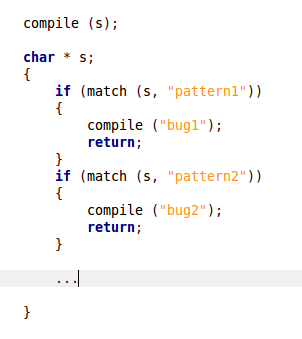
\includegraphics[keepaspectratio=true, scale=0.8]{compiler_match_pattern.png}
\end{center}
\caption{\emph{Compiler checking on patterns in the compiling process}}
\end{figure}

The additional code within the compiler not only checks for login patterns any more, but also for a pattern, that tells him that the compiler is about to compile a compiler.

So we are looking at three possibilities right now, of how some code will be compiled. Most of the time no patterns will match, so the compiler will work as desired and compile just the source code that comes in. In the next case the malicious code will find a pattern that matches a login command within the to be compiled source code. In that case it will insert the Backdoor into the program. In the next and last case, the malicious code will find a pattern that matches a compiler. So we now know, that the final output will be a compiler itself. Here the malicious code will replicate itself and insert a reproduction of its own source code into the syntax tree of the to compiler be compiled.

The new compiler will act exactly as the one we are talking about. The compilers source code itself is clean but it still contains Backdoors which we can not easily check or find.

For example if ten years ago someone implemented a Backdoor in a popular compiler such as the gcc C compiler, we will not find any clue of a Backdoor in the last dozen compiler versions of the compiler or compiled programs. Millions of computer systems could still be infected with a Backdoor.

\newpage

\subsection{How to implement one}

To fully understand the principle of a Backdoor compiler we start from scratch by looking at self reproducing programs. A self reproducing program can print out its own complete source code. 

Because of the ability to print out the own source code, a self reproducing program can of course deliver an unlimited amount of additional baggage (e.g. source code).

There are different attempts to write self reproducing programs. We will look at one quite short example in C that works with substitution.

\begin{figure}[h]
\begin{center}
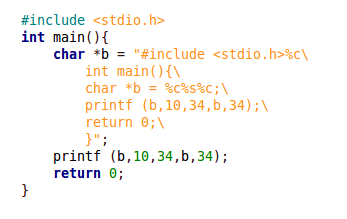
\includegraphics[keepaspectratio=true, scale=0.8]{Simple_Self_Reproducing.png}
\end{center}
\caption{\emph{Simple self reproducing program}}
\end{figure}

We mainly just define a char pointer (similar to a char array, it represents a string in the C language) in which we copy \& paste all the code we wrote. In the next step we have to substitute every special character like the " or \textbackslash n because it would terminate the string (at least after printing it out into a new source code file). We simply substitute it with a \emph{\%c} for each special character. 

After that we call a print routine to print out the own source code. In C printing works with substitution as well. So we basically print the copy \& paste version of our own source code and substitute every \emph{\%c} with the ascii representation of ", which is 34 or \textbackslash n, which is 10. And, to get it self reproducing again for the next version as well, we print the string without substitute special characters for the inside \emph{char *} definition.

This example is most simple, but obviously one can write highly complex programs by just defining the \emph{char *} at the beginning, copy \& paste the whole source code and substitute all appearance of " and \textbackslash n.
\\
\\
In order to generate a Backdoor compiler, simple self reproduction is noct sufficient. Depending on the source code to be compiled, the Backdoor compiler has to show different behaviour.

Inside a compilation process, the compiler is now checking the incoming code on specific patterns. The compiler has to at least distinguish between three different patterns. One, that tells him, that the code is just random and not of particular interest, the Backdoor compiler then does nothing and compiles correctly. One, that tells him, the incoming code matches for example a login-function. In this case the malicious compiler inserts the Backdoor into the parse tree. And the last pattern which matches compiler to be compiled. In that case the compiler prints its own source code like shown above into the parse tree of the new compiler.

The last and final step is to use the malicious compiler, to compile its original source code (without our Backdoor). Once the backdoored source code is deleted, there is no trace of our Backdoor anywhere anymore.
\\
\\
The code example below demonstrates this behaviour.

\begin{figure}[h]
\begin{center}
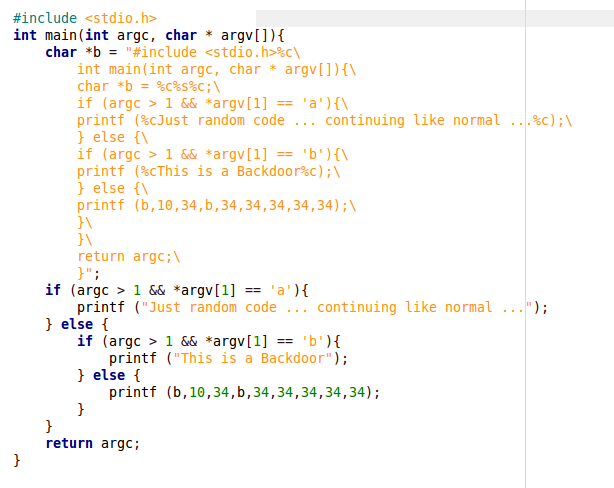
\includegraphics[keepaspectratio=true, scale=0.8]{Complex_Self_Reproducing.png}
\end{center}
\caption{\emph{Complex self reproducing program}}
\end{figure}

The first part of the code above is, like in the first short code example, a copy \& paste version of the whole program. After that the program just checks the incoming argument \emph{argv} on its value.

If the first argument is a string starting with the character `a', we assume, it matches no specific pattern and print out \emph{`Just random code ... continuing like normal ...'}.

If the string starts with `b' we assume that a pattern matches for example a login command. In this case we print out: \emph{`This is a Backdoor'}.

In all other cases, assuming we are dealing with a compiler now, we print out our own complete source code by substituting all appearances of \emph{\textbackslash n} and \emph{"}.

\subsection{Thoughts on compiler testing}

We talked about how Backdoors can infect compilers on a very deep level, not easily to be found on a rough check. We will now discuss different ways of verifying compilers on different levels of complexity.

\subsubsection{Write a new compiler}

This is the most straight foreward and safe way to be sure no Backdoor is anywhere in compiled programs. The downside of writing a new compiler is, that it takes time and knowledge to write. And if there is any existing compiler/interpreter or software used to create the new compiler, they must be verified too. It does not help much if the new compiler gets inserted the Backdoor using an infected existing compiler.

There are some ways to write and bootstrap a compiler from literally nothing[11]. This way there is certainly no Backdoor in the compiler. This method is also very time consuming and complex.

\subsubsection{Testing compilers through obfuscation}

A very simple approach to verify or compile a trusted compiler version could be, to use an obfuscater, a program that takes code as input and gives an output, that varies the code in a way the compiler compiling that obfuscated code does not recognize specific patterns. That includes changing names, procedures, variables and syntax of the code by not changing the semantics of the code in any way.

So if the code compiles now, the compiler (if checking for syntactic patterns) would not recognize the code as a login-command and compiles it correctly. Note, that this program could probably going to be very inefficient because of no optimizations done by the compiler.

For instance taking the source code of an existing compiler (which is, of course, clean), obfuscate it and let it be compiled by an existing unstrusted compiler.
Then one take the new inefficient compiler to compile the source code again. Since using the obfuscater before, the backdoor is probably not inserted in the non optimized compiler which now can compile the real compiler without passing any backdoor on to it.
However one can never be sure that it actually worked.

There are a few variables to its actual functionality too. For example the obfuscator could be infected by the compiler and recognize the patterns itself or is just not good enough to obfuscate the program, so the compiler will not recognize patterns.

The bigger problem is, that we assume that the backdoor implementation is very simple and just scans for syntactical patterns, for example for a procedure called `login`. 
An intelligent backdoor implementation, in contrast, is not just checking for specific names (they could be changed in newer operating system distributions or versions) but more likely checking the parse tree built by the compiler after the lexical analysis during the syntactic analysis. As long as the code syntactics remain the same and match the tree the backdoor can be inserted. The semantics stay the same after obfuscating the code. During the process of obfuscating only the syntactics going to be changed.

To go further, the problem of comparing the semantics of two programs can be reduced to a NP-hard problem, called the `halting problem'[12].
That means, it is widely accepted that it is not possible to solve that problem at all.

\subsubsection{Verification by auditing machine code}

It is possible to reverse engineer the code, and check, what it does. Despite the fact of being sure whether a Backdoor exists or not, by choosing this method, it is for sure one of the most time-consuming methods for achieving this aim.
Because of missing the Backdoor completely is still possible.

It actually would not be completely unrealistic that the malicious Backdoor in the compiler could even subvert the re-engineering by subverting the re-engineering tools.

\subsubsection{Compiler bootstrapping test}

Bootstrapping[7] refers to a compiler in which the source language is identical with the implementation language. Bootstrapping is normally used to compile compilers by using existing compilers. If one need a compiler for a specific machine code, we use a compiler which compiles the source code of the existing compiler to the desired machine code language.

Each compiler can be represented as a T-diagram as in \emph{Figure 4}.

\begin{figure}[h]
\begin{center}
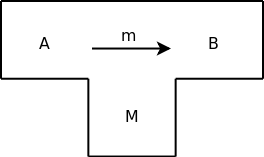
\includegraphics[keepaspectratio=true, scale=0.4]{T_diagram_sample.png}
\end{center}
\caption{\emph{T-diagram representing a compiler}}
\end{figure}

This diagram shows a compiler \emph{m}, which is written in the language \emph{M} and and compiles from language \emph{A} to language \emph{B}. This is all we have to know right now.
We can now apply compilers to each other's source code to get compilers in different languages. When we apply a compiler \emph{C2} to a compiler \emph{C1} we will get an output compiler called \emph{C3}as shown in \emph{Figure 5}.

\newpage

\begin{figure}[h]
\begin{center}
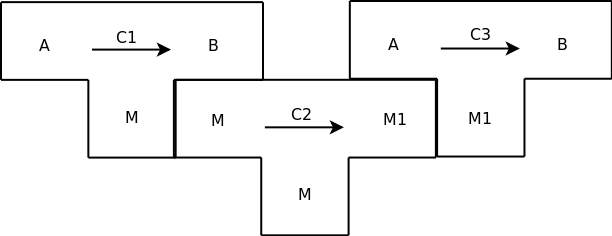
\includegraphics[keepaspectratio=true, scale=0.4]{T_diagram_apply.png}
\end{center}
\caption{\emph{C2 applied to C1, resulting in C3}}
\end{figure}

Compilers \emph{C1} and \emph{C3} are identical except the implementation language which is compiled from \emph{M} to \emph{M1} by \emph{C2}.
\\
\\
The actual algorithm of the bootstrapping test is now to take a compiler \emph{Csl} we would like to validate. It is written in the language \emph{Sl} and compiles \emph{Sl} to \emph{Tl}. We now take an existing compiler \emph{m0} which compiles \emph{Sl} to \emph{Tl} and apply it to the implementation language of the to be verified compiler \emph{Csl}. The resulting compiler \emph{m1} is now written in \emph{Tl} and otherwise identical to \emph{Csl}, thus can be applied to the implementation language of the original compiler \emph{Csl}. This chain can go on for a while. Assuming \emph{m0} works correctly and \emph{Csl} does too, then applying it to itself should reproduce character by character the same compiler again: example \emph{Figure 6}.

\begin{figure}[h]
\begin{center}
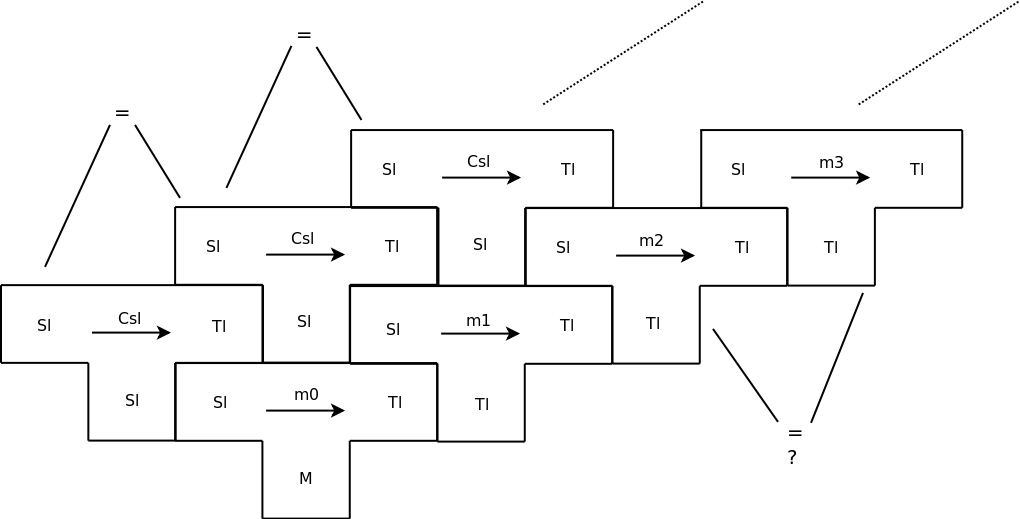
\includegraphics[keepaspectratio=true, scale=0.4]{T_diagram_bootstrapping.png}
\end{center}
\caption{\emph{Compiler output verification}}
\end{figure}

The assumption on this test is, that the compiler just reproduces itself in the right way if it is working correctly and contains no Backdoor.
This works, assuming that any Backdoor would alter the output of the compiler in specific situations. If the compilers output is altered at some stage, the character by character comparison will then fail and one know that somehow the compiler does not work correctly.

One down side is, that a compiler which compiles some language feature wrong but this feature is not used in the compiling process itself, the code will always be identical, but the compiler could still be working incorrectly on some parts or contain Backdoors.

The problem with this assumption is, that the Backdoor might be inserted at the exact same spot in the parse tree every time again. First by \emph{m0}, which is trusted. If \emph{m0} does not contain the Backdoor, the results \emph{m1}, \emph{m2}, \emph{m3} \emph{...} will be correct, but \emph{Csl} will not because in this case we do actually more something like a source level testing, then low level verification here.

The bottomline on the bootstrapping test is then, that it is probably useful for normal compiler testing, but not much of use to find well implemented hidden Backdoors in the machine code.

\subsubsection{Diverse double compiling}

Diverse double compiling[10] is finally a way to make a hundred percent sure a specific compiler does not contain any form of Backdoor. It is similar to the bootstrapping test in the previous section, but expands it by bit-for-bit checks of the binary outputs.

The principle is to recompile the source code of the compiler two times. First with a compiler that has already proved secure and does not contain any form of payload, second with the output from the first compilation. In the next step you do a bit-for-bit comparison in a secure environment on the original untrusted binary and the second compilation.

If these two files are exactly the same, then the compiler is proved not to contain any Backdoors.

I will not go further into that concept because doing a diverse-double-compiling-check on a compiler requires and depends on a lot of preconditions that are quite hard to realize.

You need for example a compiler which is already bug-free, you need a proven safe environment which does not interfere with the compilation and comparison opertions. The existing safe compiler even has to translate to the same byte-code like the one we want to check on, compiling the same language constructs. 

I am convinced to say, that if we meet all these security requirements, and do already have a safe working compiler, compiling the same semantics on same language constructs, we do not necessarily have to verify another, quite similar compiler.

\newpage

% -----------------------------------------------------------------------
% Examples of Backdoors

\section{Examples of Backdoors}

There are some examples of real existing Backdoors out there. But the most impressive one, in my opinion, is still the Backdoor compiler. There are rumours Ken Thompson, the inventer of the Backdoor compiler, actually implemented the exact Backdoor, we have been talking about. Apparently, the infected Compiler never left a secured area inside the Bell Labs but could not even be found and destroyed within. The example was made on a Linux login-command and the Backdoor was implemented in a GNU C-compiler. It behaved exactly how we stated and even covered itself against being found by changing the disassembler
\\
\\
Another example of a Backdoor which nearly could have made it out to release was implemented into the Linux kernel. It was basically just a two-line change, an \emph{if}-statement which checks, if two different flags were set and do something.

The only change here was, that the initial equals check on administration mode \emph{==} was changed to \emph{=}, what actually not checks if you are administrator, but gives you root access inside the \emph{if}-statement.

The smart part of this Backdoor was to find two flags that would go together without causing an error, but would not go together normally. In that case everyone with knowledge of the combination of those flags would then be able to gain root access over the system.

A routine integrity check on that file was called because someone manually edited the file. During that check later on someone then found the Backdoor and called in an investigation.[3, 4]
\begin{mySourceCode}
\normalsize
\begin{Verbatim}[samepage=true]
if ((options == (__WCLONE|__WALL)) && (current->uid = 0))
    retval = -EINVAL;
\end{Verbatim}
\end{mySourceCode}
A last, but very interesting example is about a program only designed to work as a Backdoor. The program is called \emph{Backdoor.OptixPro.12}. Its only use is to get some attacker complete remote control over a Microsoft Windows machine. It disables antivirus-programs and firewalls and allows the attacker to record keystrokes. According to the author, this program has been downloaded over 270 000 times until some hackers found out about a hidden encrypted password hardcoded in the program's binary. In that case the the programmer backdoored the backdoor program.

\newpage

% -----------------------------------------------------------------------
% Conclusion

\section{Conclusion}

In conclusion we see, that it is not very difficult to design malicious software if you put your mind to it, as we have seen in those short source code examples, but it is incomparable more complicated to ensure some software is clean, containing no bugs or malicious code. We have seen, that even testing programs is complicated.

The most important fact is, that even if your source code is fine, the result can still not be trusted because of the kind of Backdoors discussed in this paper.

The real threats are sometimes not to be found on source level but on a much deeper level. Most people and companies tend to forget that bugs or Backdoors, the deeper they get, the more power they could have and the less likely you will be able to find them.
\begin{quote}
`The moral is obvious. You can't trust code that you did not totally create yourself. (Especially code from
companies that employ people like me.) No amount of source-level verification or scrutiny will protect you
from using untrusted code.'
\end{quote}
\emph{(Ken Thompson, Reflections on Trusting Trust, 1984)}
\newpage

% -----------------------------------------------------------------------
% References

\section{References}

\begin{enumerate}

\item{Apple Computer Inc. (2006), Small Number of Video iPods Shipped With Windows Virus. \\http://www.apple.com/support/windowsvirus/.}
\item{Andy Patrizio (2007), Virus Infections Reflect Sloppy Manifacturing\\ http://www.internetnews.com/security/article.php/3711266}
\item{Larry McVoy (2003), BK2CVS problem.\\http://lkml.indiana.edu/hypermail/linux/kernel/0311.0/0635.html}
\item{Kevin Poulsen (2003), Thwarted Linux backdoor hints at smarter hacks\\http://www.securityfocus.com/news/7388}
\item{Kevin Poulsen (2004), Backdoor program gets backdoored\\http://www.securityfocus.com/news/8893}
\item{Nicholas Weaver, Vern Paxson, Stuart Staniford, Robert Cunningham (2003), A Taxonomy of Computer Worms\\Copyright 2003 ACM 1-58113-785-0/03/0010\\http://citeseerx.ist.psu.edu/viewdoc/summary?doi=10.1.1.10.4743}
\item{Wolfgang Goerigk (1999), On Trojan Horses in Compiler Implementations\\Institut fur Informatik und Praktische Mathematik\\ISBN:3-642-11511-X 978-3-642-11511-0\\http://citeseerx.ist.psu.edu/viewdoc/summary?doi=10.1.1.20.3206}
\item{Ken Thompson (1984), Reflections on Trusting Trust\\Reprinted from Communication of the ACM, Vol. 27, No. 8, August 1984, pp. 761-763. Copyright © 1984,\\http://citeseerx.ist.psu.edu/viewdoc/summary?doi=10.1.1.84.8238}
\item{Samuel T. King, Joseph Tucek, Anthony Cozzie, Chris Grier, Weihang Jiang, and Yuanyuan Zhou\\Designing and implementing malicious hardware\\University of Illinois at Urbana Champaign, Urbana, IL 61801\\published: USENIX Association Berkeley, CA, USA ©2008\\http://citeseerx.ist.psu.edu/viewdoc/summary?doi=10.1.1.143.4529}
\item{David A. Wheeler (2005), Countering Trusting Trust through Diverse Double-Compiling\\ISBN:0-7695-2461-3\\www.acsa-admin.org/2005/papers/47.pdf}
\item{Edmund Grimley Evans (2001), Bootstrapping a simple compiler from nothing\\http://homepage.ntlworld.com/edmund.grimley-evans/bcompiler.html}
\item{Susan Horwitz, Identifying the Semantic and Textual Differences
Between Two Versions of a Program\\ISBN:0-89791-364-7\\http://dl.acm.org/citation.cfm?id=93574}
\item{Bartosz Bobkiewicz (2003), Hidden Backdoors, Trojan Horses and Rootkit Tools in a Windows Environment\\http://www.windowsecurity.com/articles/\\hidden\_backdoors\_trojan\_horses\_and\_rootkit\_tools\_in\_a\_windows\_environment.html}
\item{Adam L. Young (2004-2006), RSA Labs Cryptography FAQ version 4.1\\http://www.cryptovirology.com/cryptovfiles/cryptovirologyfaqver1.html}

\end{enumerate}

All references and links were collected in September 2012.

% =======================================================================

\end{document}

